%CHKTEX-FILE 46
%\section*{Annex}
%\label{sec:appendix-OPL}
%\setcounter{section}{0}

% \subsection*{Appendix 1}
% \begin{figure}[H]
%     \centering
%     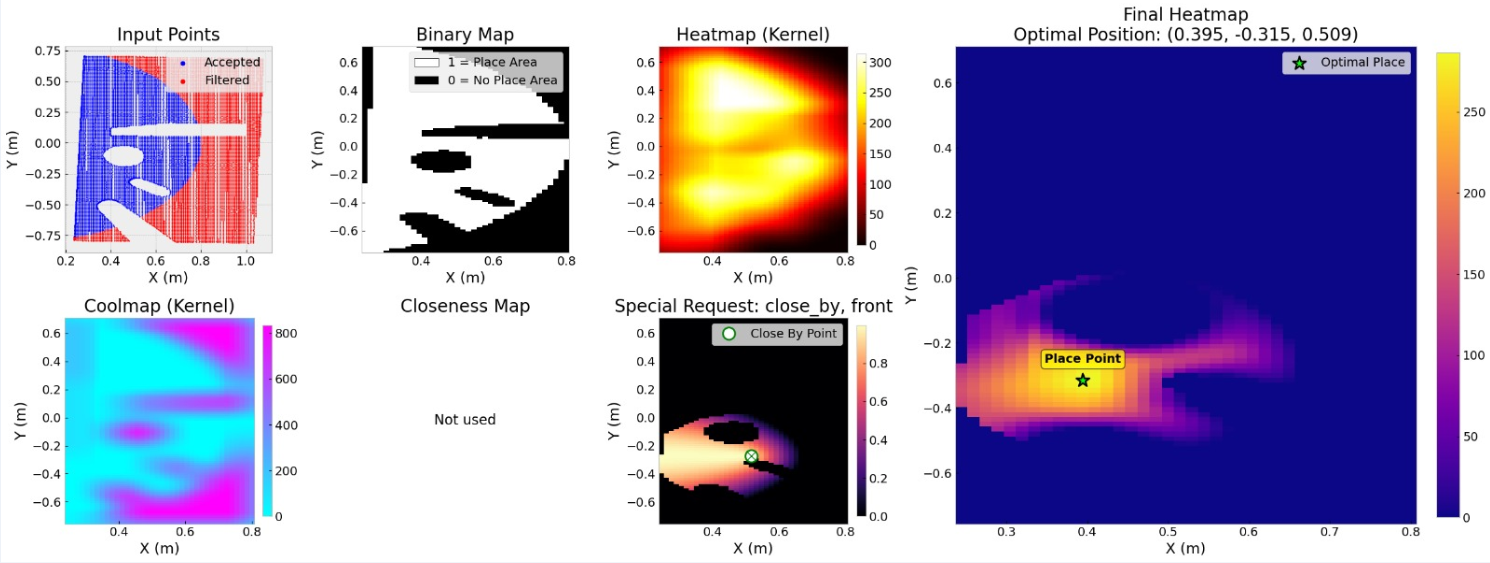
\includegraphics[width=1\textwidth]{TDPTemplate-master/images/HeatMaps.png}
%     \caption{Heatmaps generated to attend a request to place an object in front of another one.}
%     \label{fig: heatmap}
% \end{figure}

% \subsection{Pipeline}
% \begin{figure}[H]
%     \centering
%     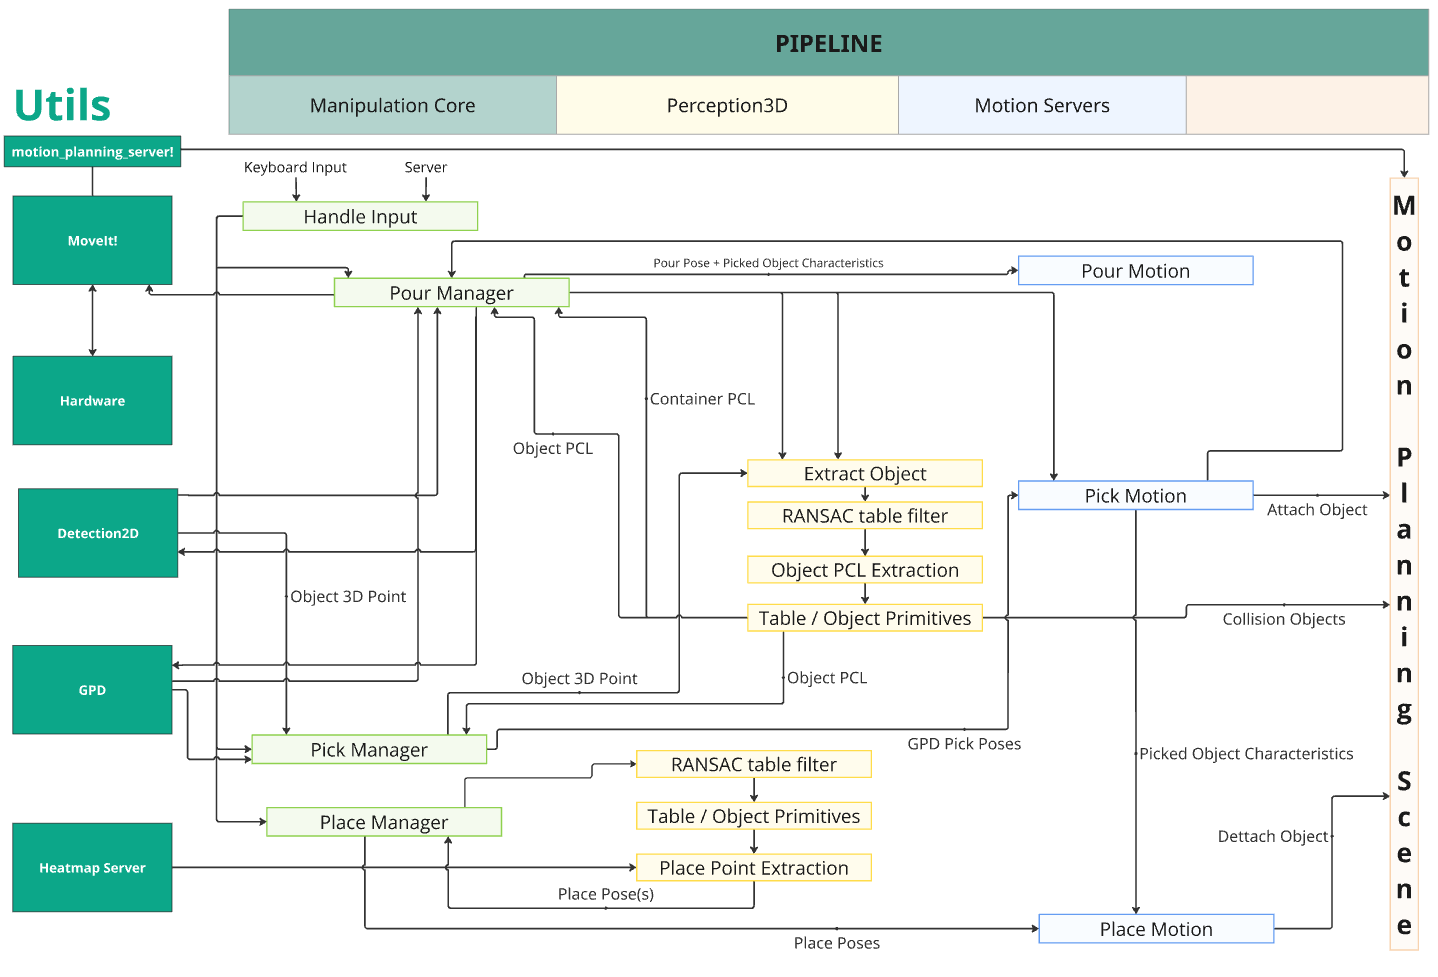
\includegraphics[width=.7\textwidth]{TDPTemplate-master/images/ManpulationPipeline.png}
%     \caption{Manipulation Pipeline with Pick, place and pour in Ros2}
%     \label{fig: manipPipeline}
% \end{figure}

% \subsection*{Appendix 2}
% \begin{figure}[H]
%     \centering
%     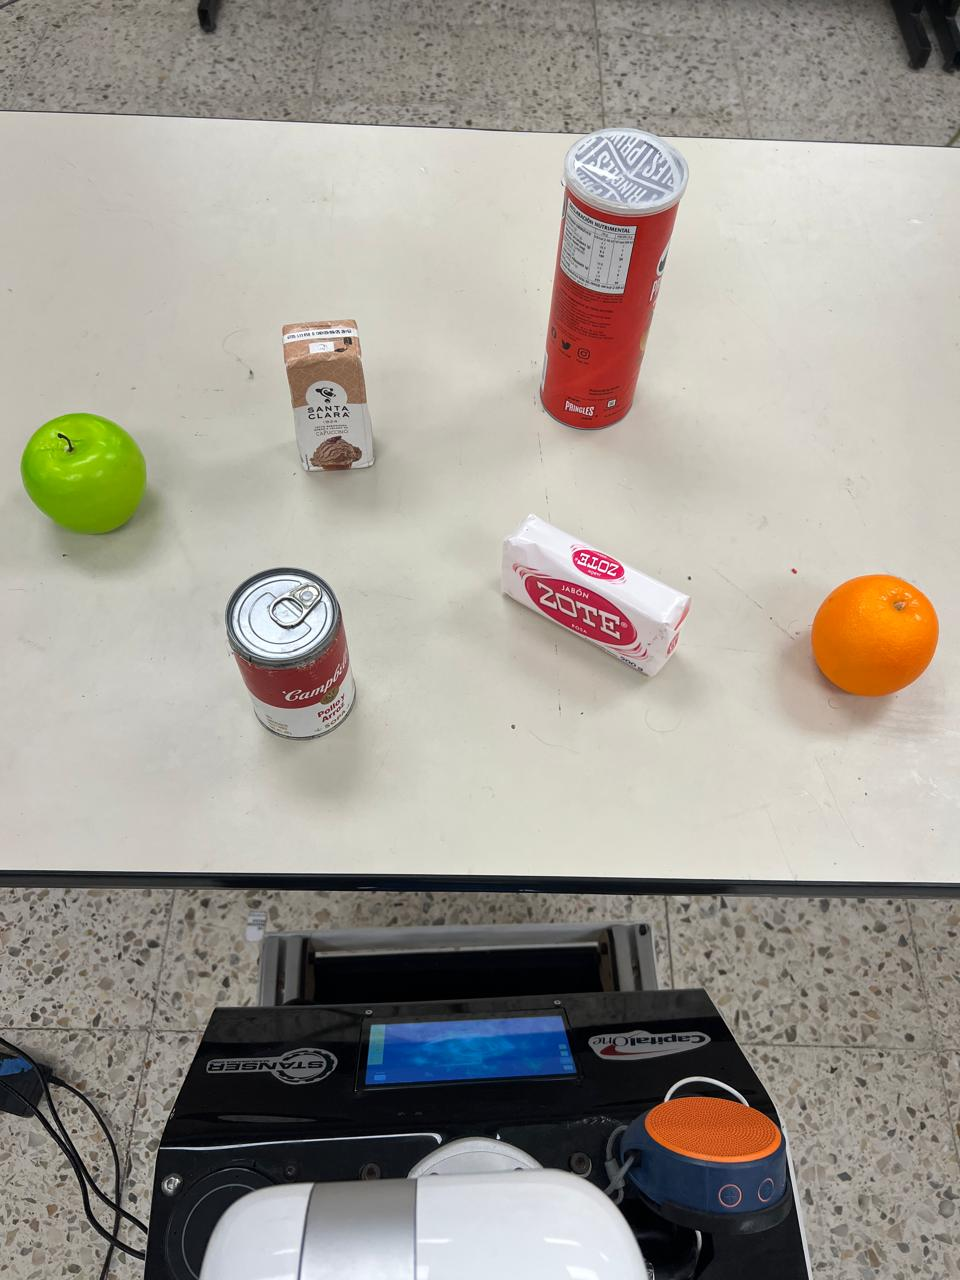
\includegraphics[width=0.55\textwidth]{TDPTemplate-master/images/pick_placeEnv.jpeg}
%     \caption{Experimental setup for Pick \& Place tasks.}
%     \label{fig:pick_place_env}
% \end{figure}

% \subsection*{Appendix 3}
% \begin{figure}[H]
%     \centering
%     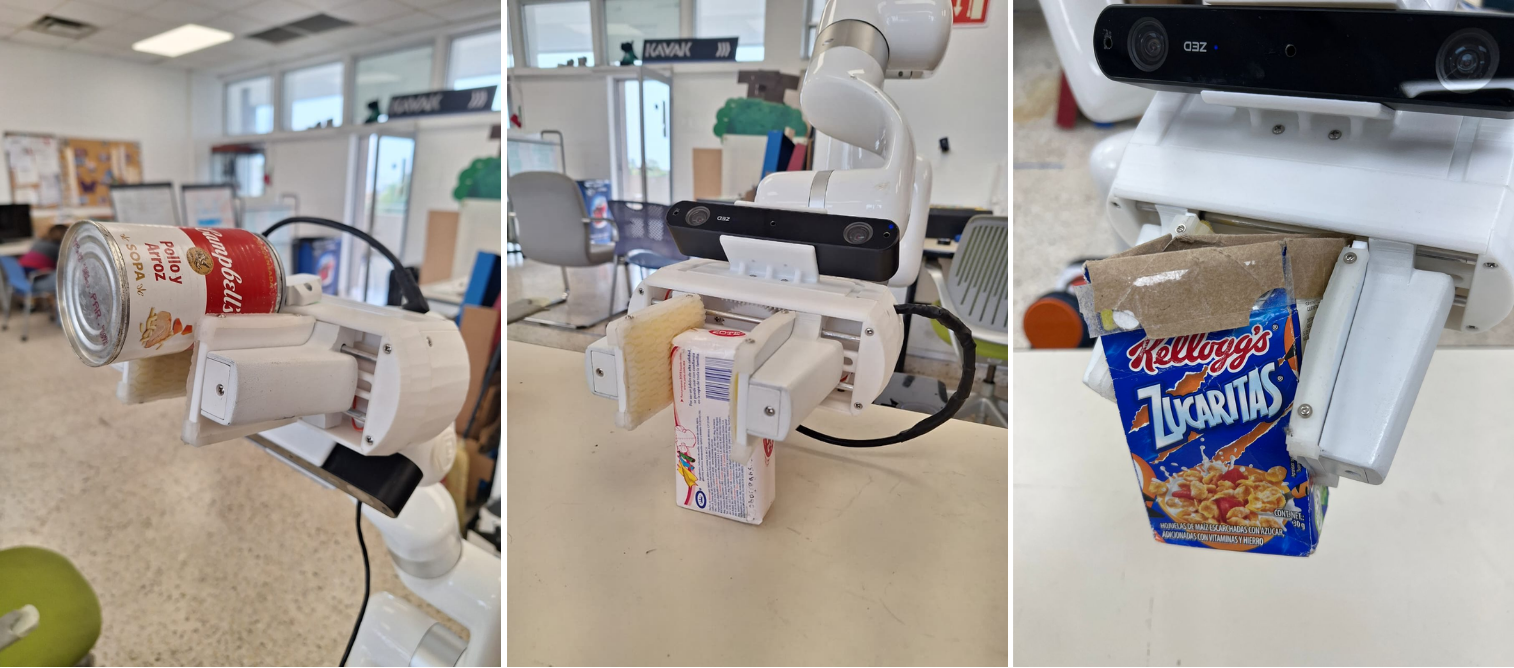
\includegraphics[width=0.95\textwidth]{TDPTemplate-master/images/gripperGraspingPositions.png}
%     \caption{Gripper grasps from different positions.}
%     \label{fig:gripperGraspingPositions}
% \end{figure}

% \section{Computer Vision}
% \subsection{Overview of the Robot’s Computer Vision Pipeline}
% \begin{figure}[H]
%     \centering
%     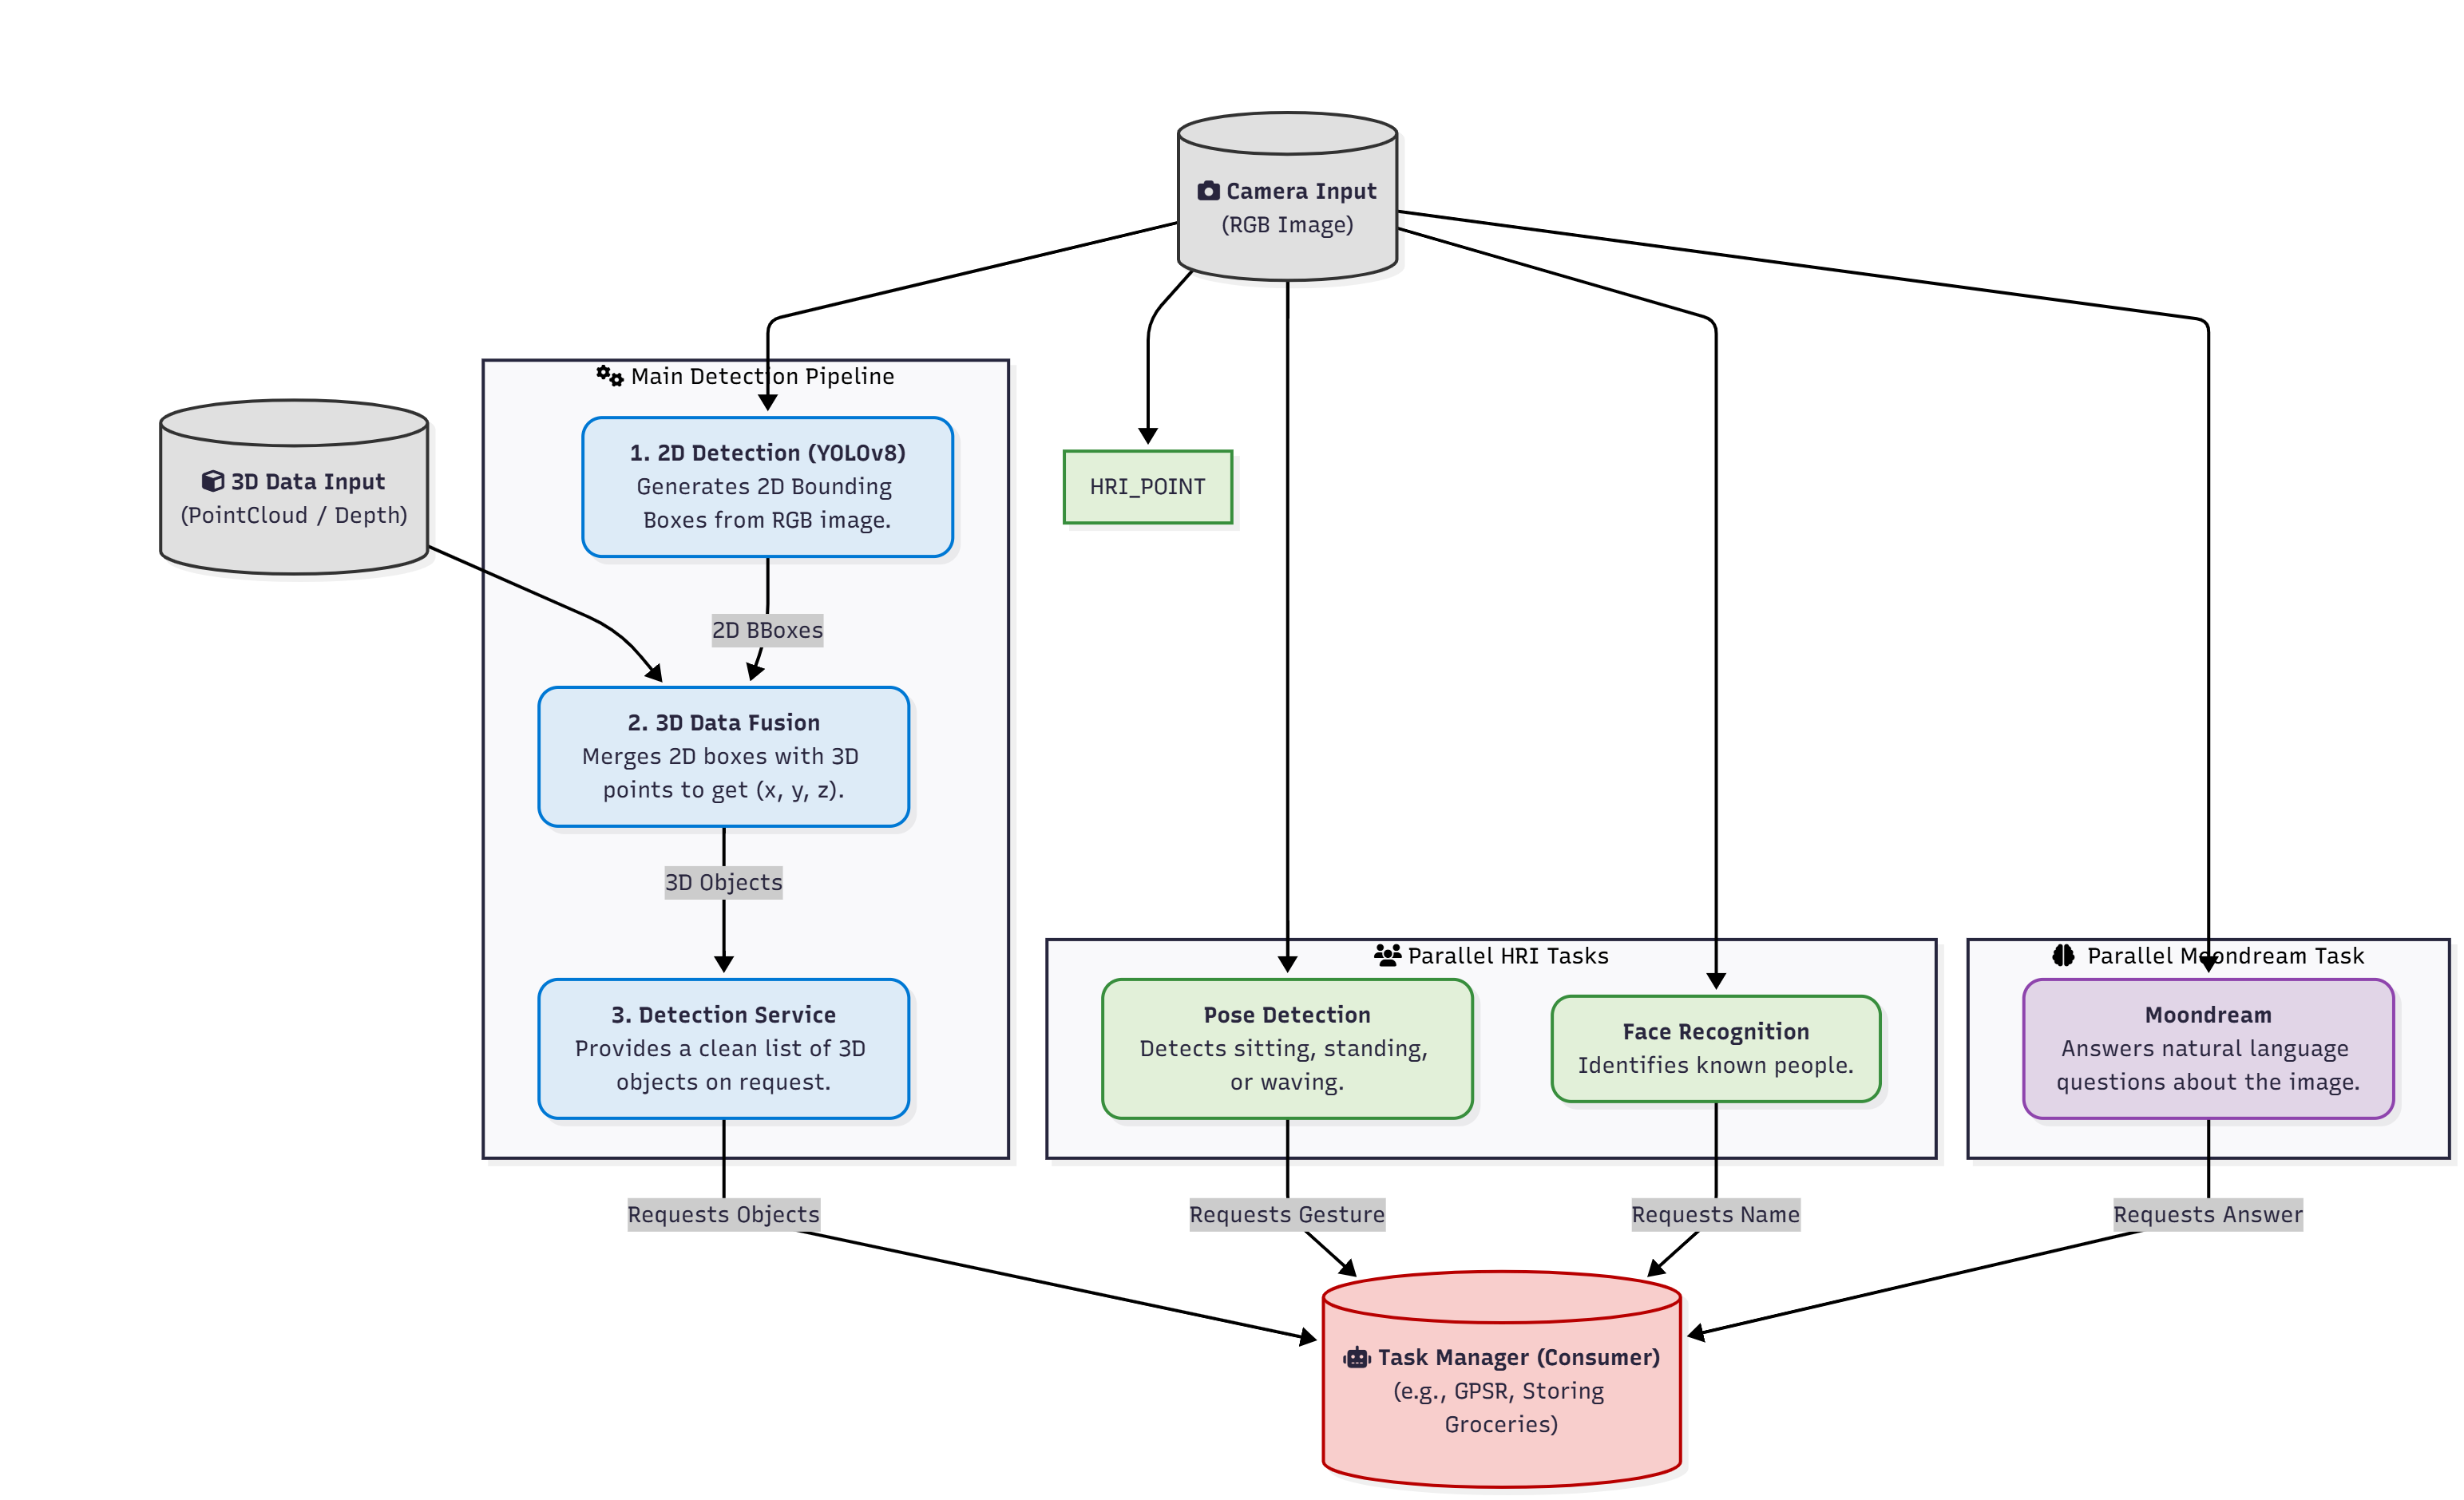
\includegraphics[width=1\textwidth]{TDPTemplate-master/images/Vision_pipeline.png}
%     \caption{Vision pipeline.}
%     \label{fig: pipeline}
% \end{figure}




% \section{HRI}

% \subsection{HRI Pipeline}
% \begin{figure}[H]
%     \centering
%     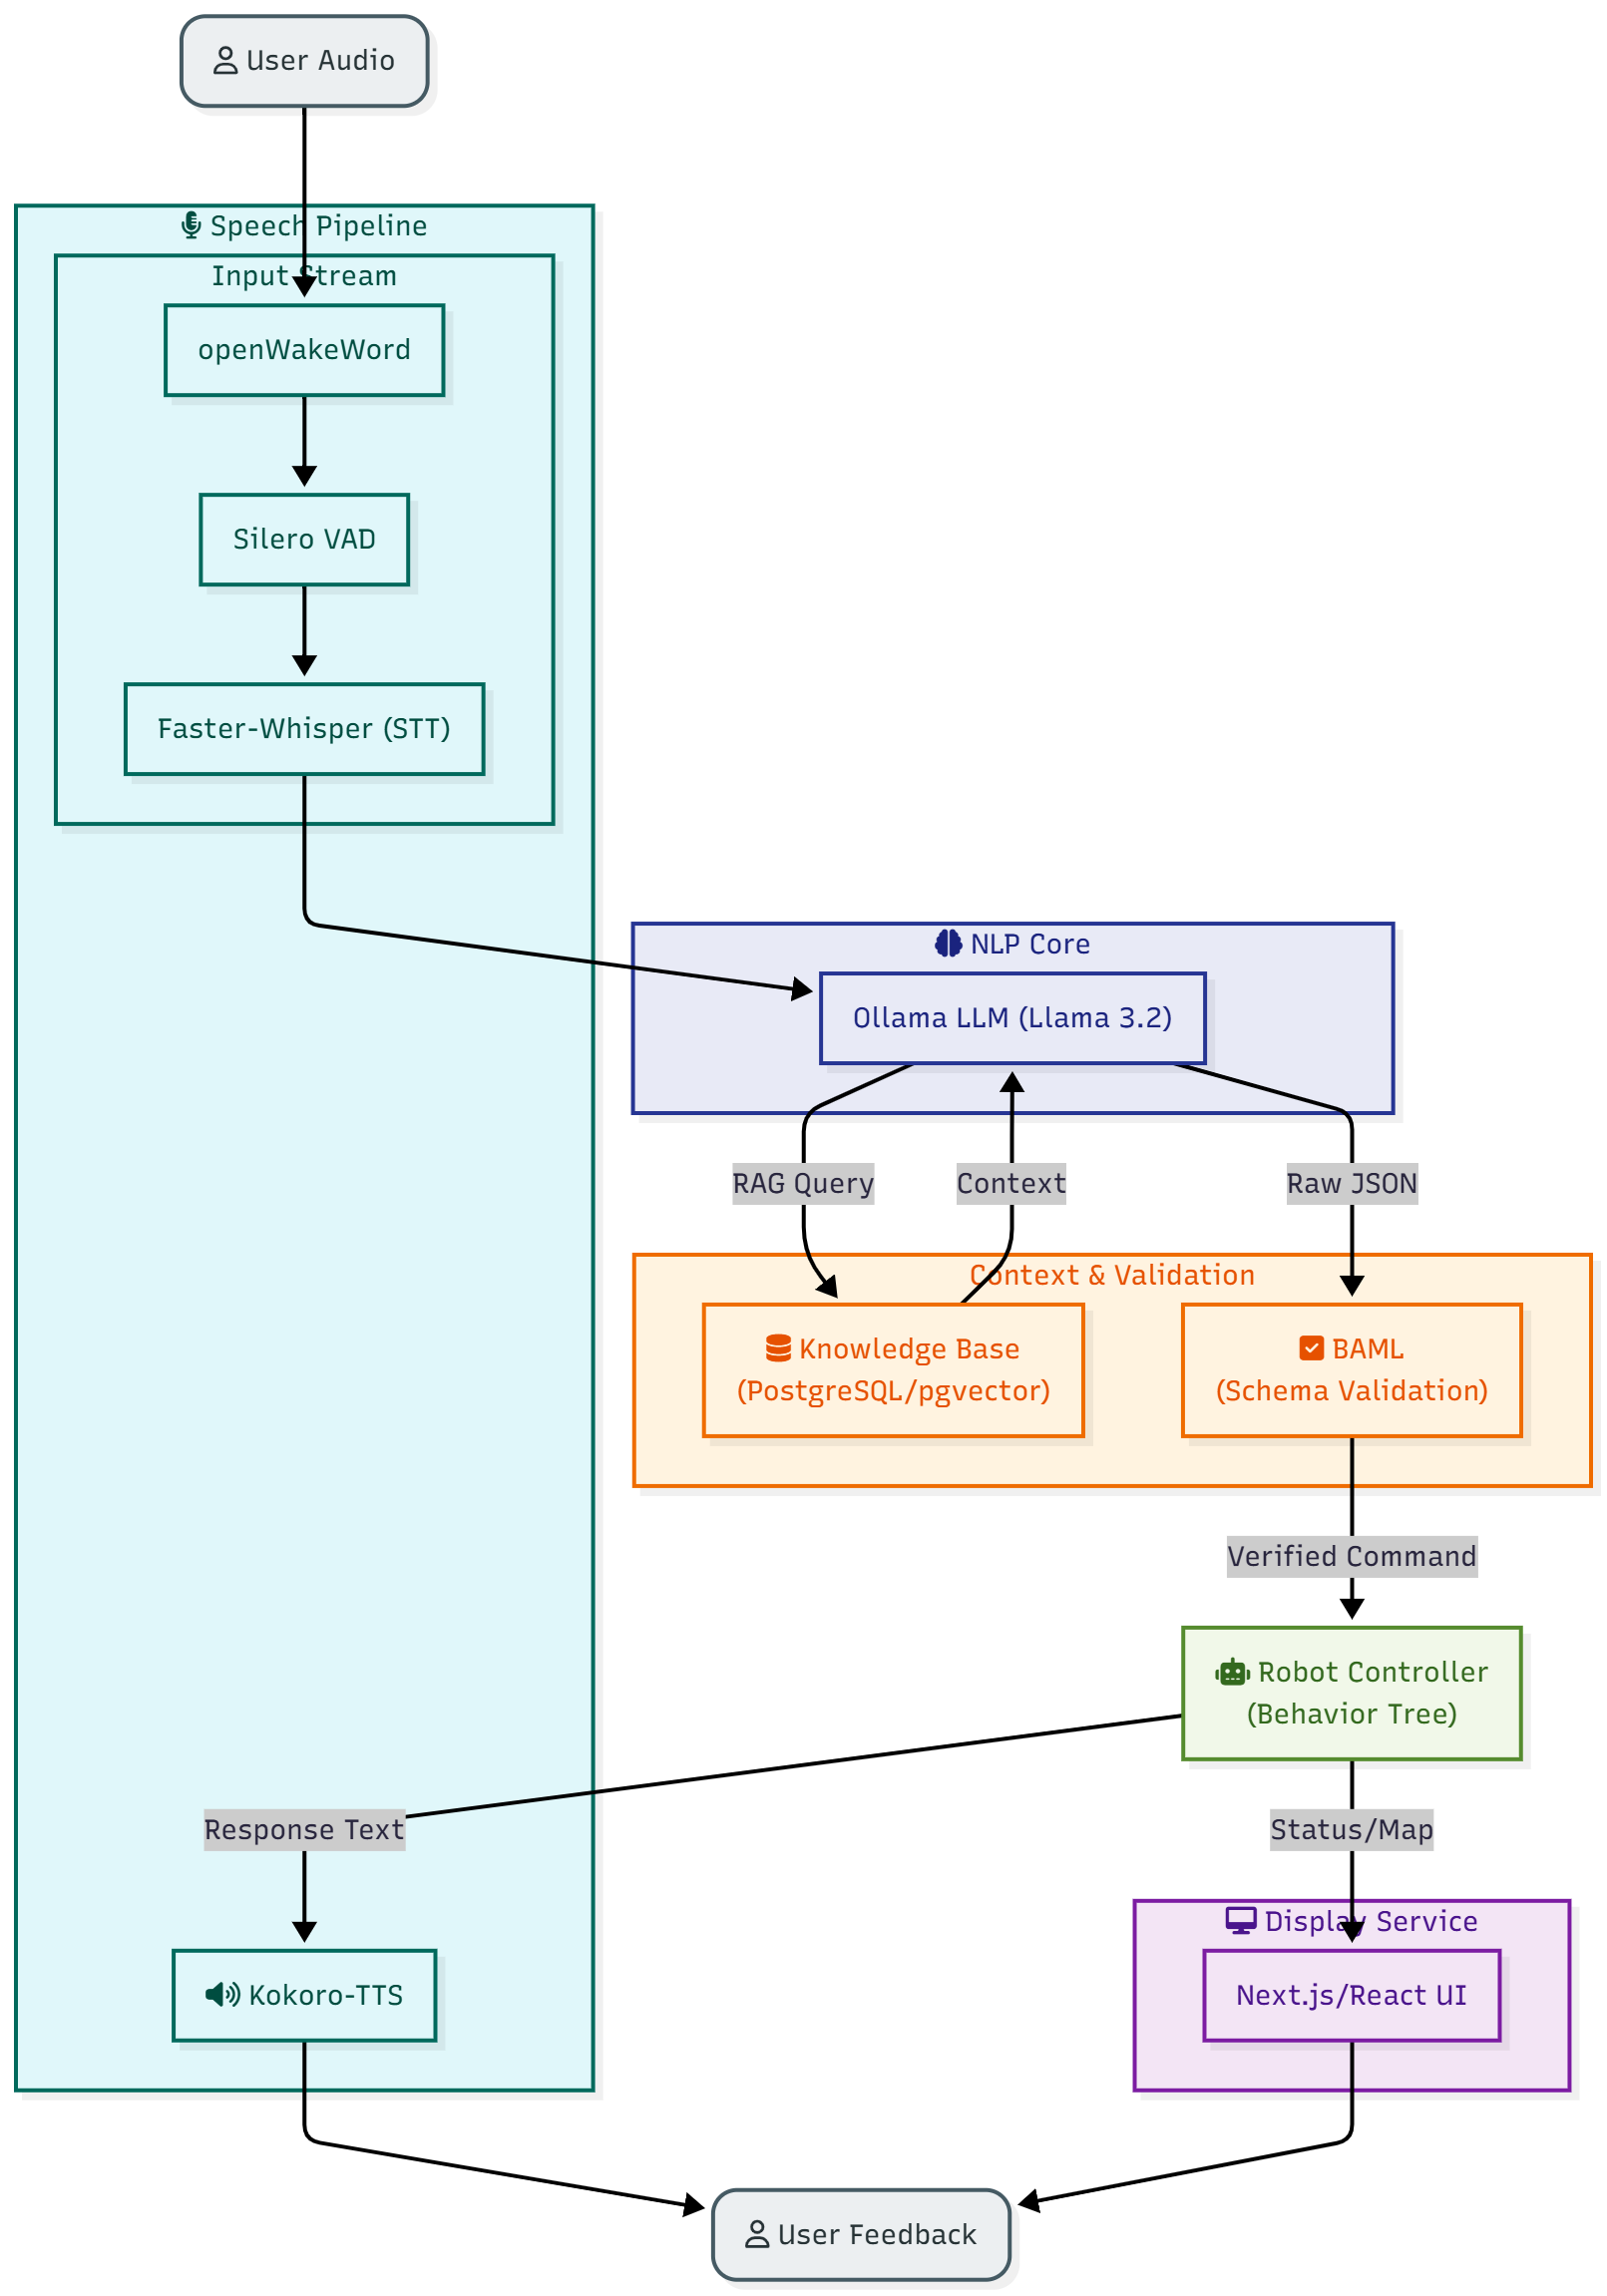
\includegraphics[width=0.6\textwidth]{TDPTemplate-master/images/HRI_pipeline.png}
%     \caption{HRI Pipeline}
%     \label{fig:hri_pipeline}
% \end{figure}

% \section{Navigation}

% \subsection{Omnibase}
% \begin{figure}[H]
%     \centering
%     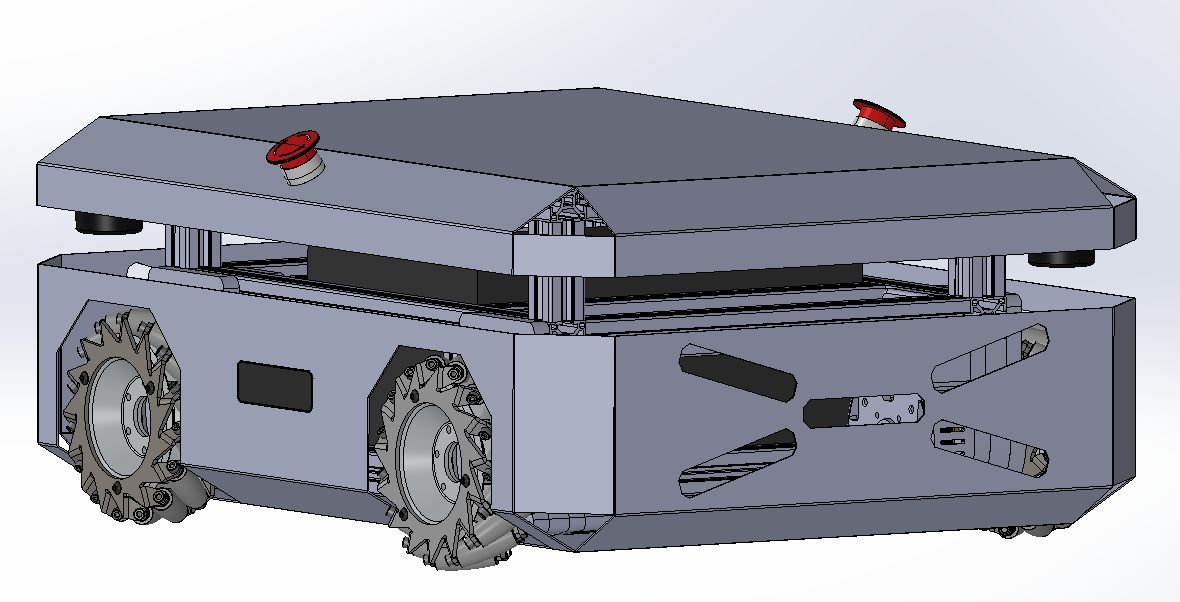
\includegraphics[width=1\textwidth]{TDPTemplate-master/images/Omnibase_CAD.jpg}
%     \caption{Omnibase CAD}
%     \label{fig:Omnibase_CAD}
% \end{figure}

% \section{Electronics}
% \subsection{PCB 3D}
% \begin{figure}[H]
%     \centering
%     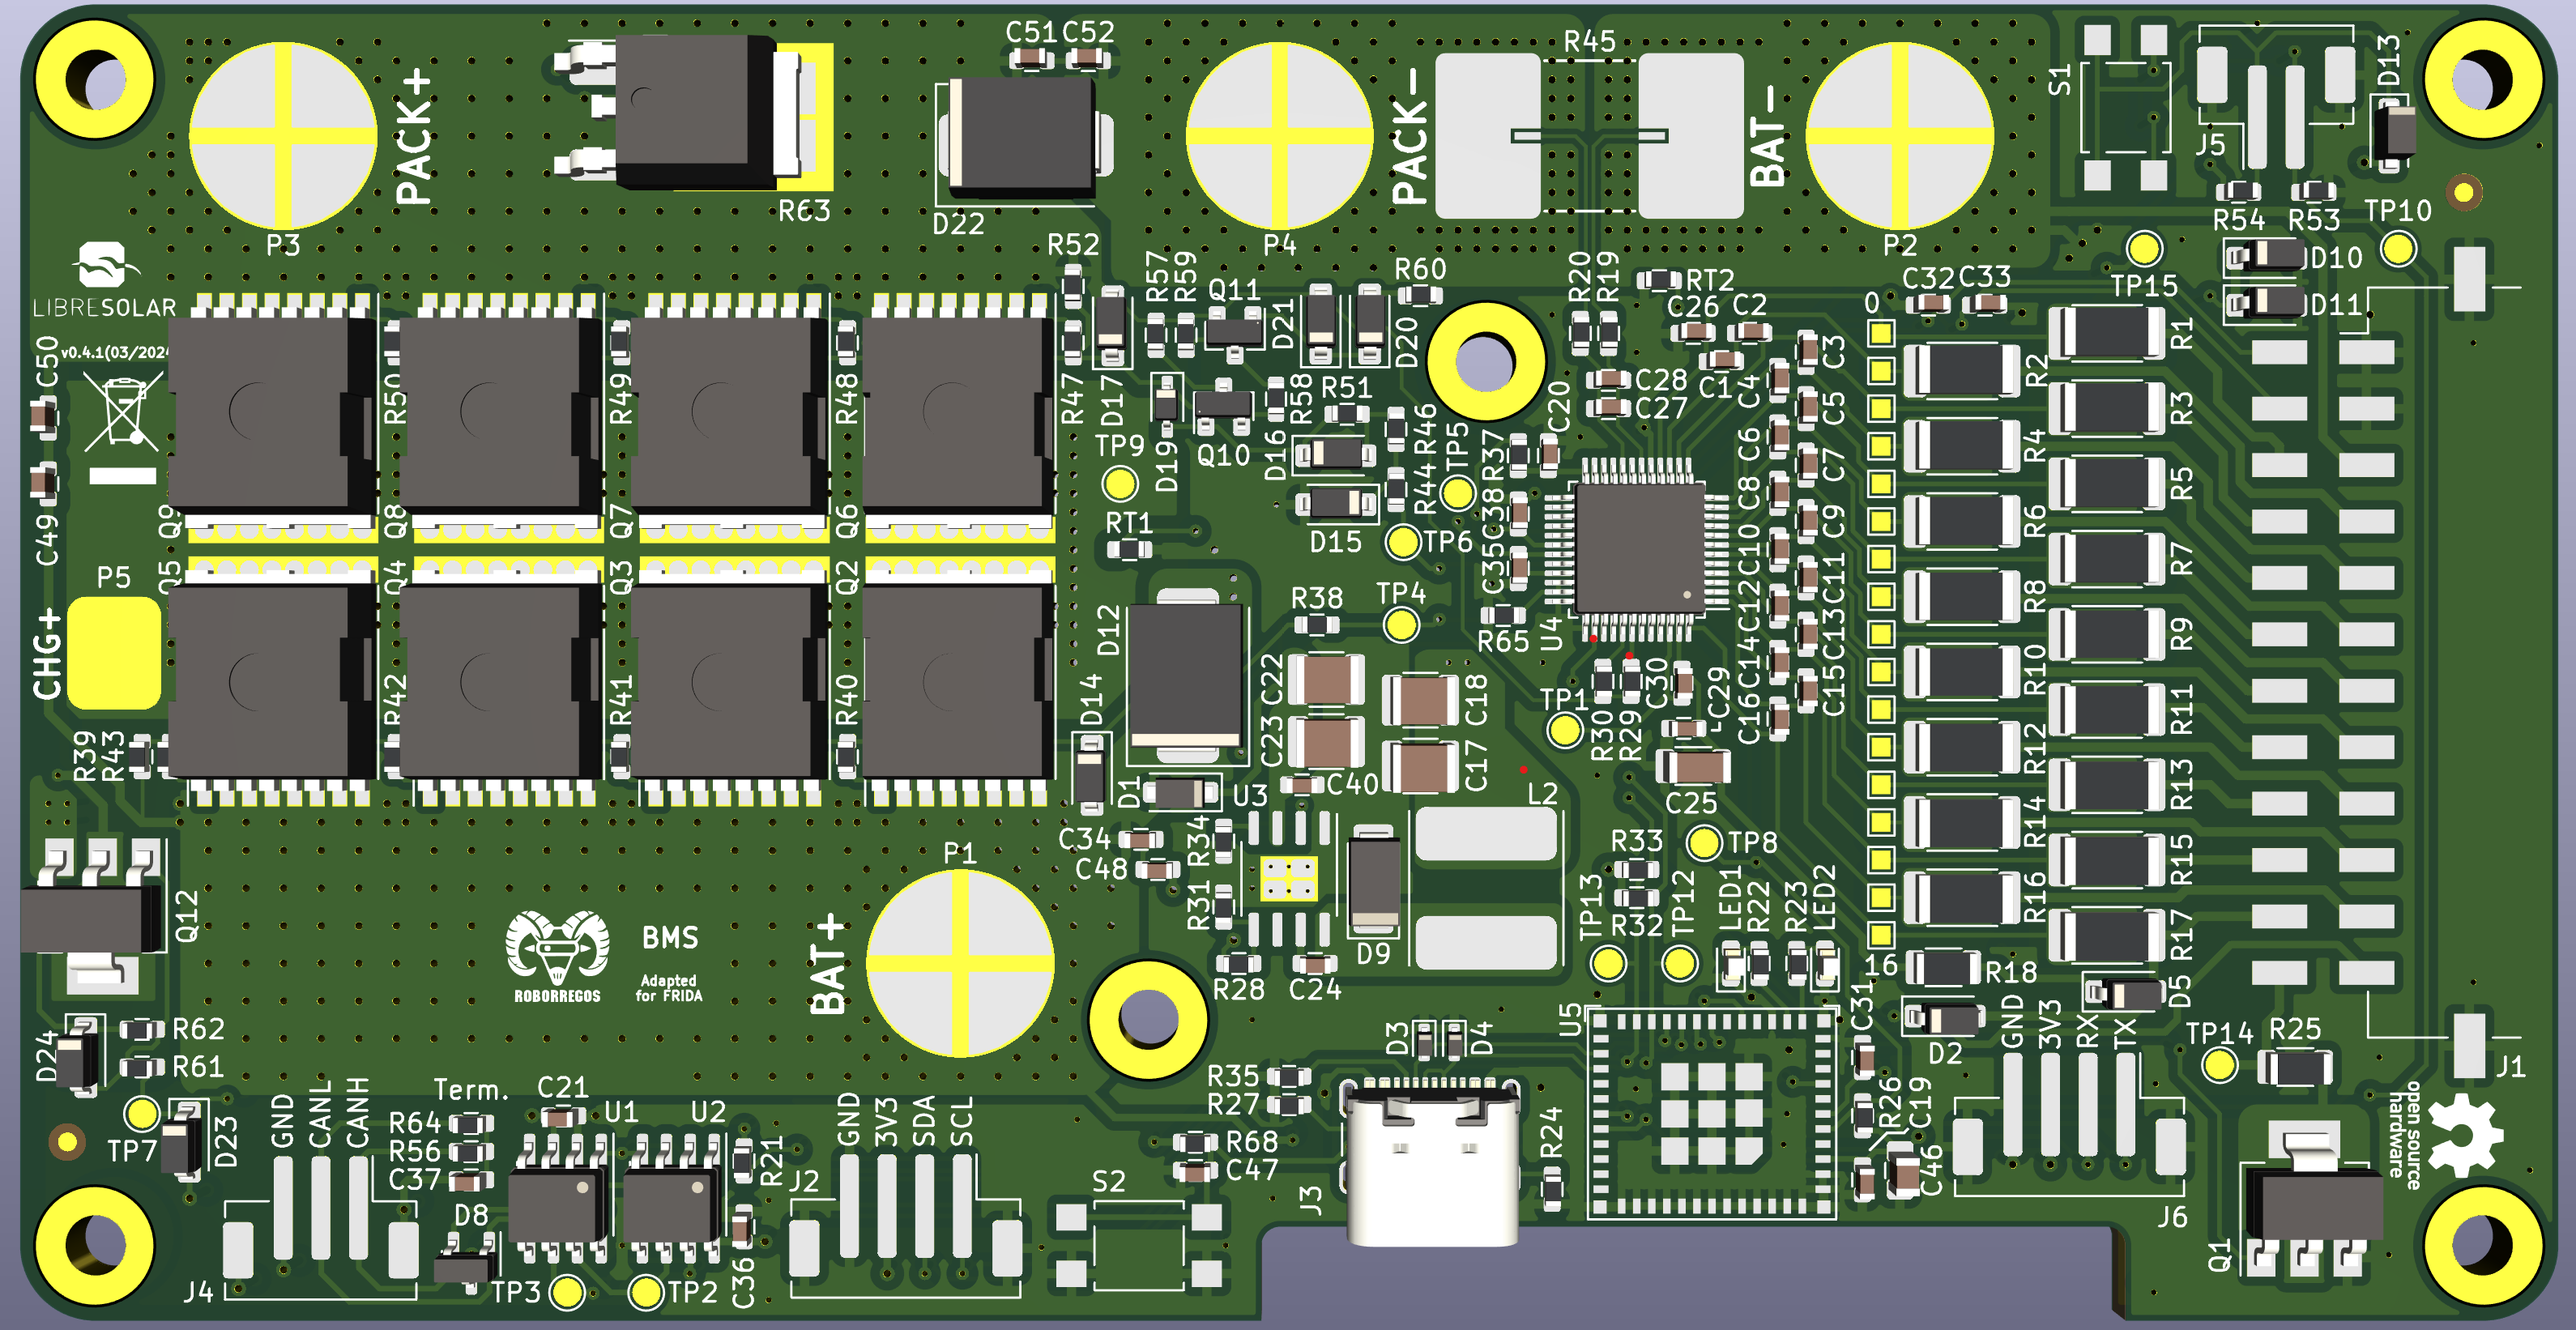
\includegraphics[width=1\textwidth]{TDPTemplate-master/images/BMS_3DView.png}
%     \caption{BMS 3D View}
%     \label{fig:BMS_3DView}
% \end{figure}